% File: memory_address_decomposition.tex
% Description: A hardcoded TikZ memory address decomposition - not generic, not
%              scalable at all.

\documentclass{standalone}
\usepackage{tikz}

\begin{document}
    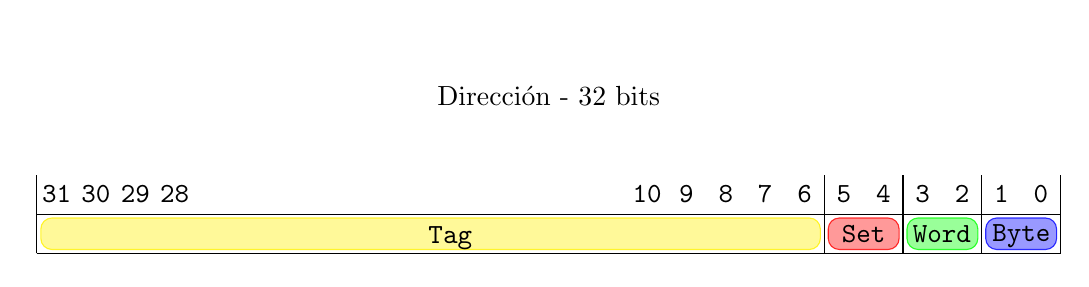
\begin{tikzpicture}
        % Grid
        \draw (0,0) -- (13,0);
        \draw (0,0.5) -- (13,0.5);
        \draw (0,0) -- (0,1);
        \draw (0,0) -- (0,1);
        \draw (10,0) -- (10,1);
        \draw (11,0) -- (11,1);
        \draw (12,0) -- (12,1);
        \draw (13,0) -- (13,1);
    
        % Bit Labels
        \foreach \a/\x in {31/0, 30/1, 29/2, 28/3, /4, /5, /6, /7, /8, /9, /10, 
            /11, /12, /13, /14, 10/15, 9/16, 8/17, 7/18, 6/19, 5/20,
            4/21, 3/22, 2/23, 1/24, 0/25} {
            \node at ({0.5*(\x+0.5)}, 0.75) {\texttt{\a}};
        }
        \foreach \a/\y in {/0} {
            \node at (0.0, {3-0.5*(\y+0.5)}) {\texttt{\a}};
        }
        
        \tikzset{block/.style = {rounded corners, #1, fill=#1!50, opacity=0.8}}
        \pgfmathsetmacro{\offset}{0.05}

        % Coloured lines
        \draw[block=yellow] (0 + \offset, 0 + \offset) rectangle (10 - \offset, 0.5 - \offset);
        \draw[block=red] (10 + \offset, 0 + \offset) rectangle (11 - \offset, 0.5 - \offset);
        \draw[block=green] (11 + \offset, 0 + \offset) rectangle (12 - \offset, 0.5 - \offset);
        \draw[block=blue] (12 + \offset, 0 + \offset) rectangle (13 - \offset, 0.5 - \offset);
        
        % Message labels
        \node at (5.25, 0.2) {\texttt{Tag}};
        \node at (10.5, 0.25) {\texttt{Set}};
        \node[right] at (11, 0.25) {\texttt{Word}};
        \node[right] at (12.01, 0.22) {\texttt{Byte}};
        
        % Title
        \node at (6.5, 2) {Dirección - 32 bits};
    \end{tikzpicture}

\end{document}

